%%%%%%%%%%%%%%%%%%%%%%%%%%%%%%%%%%%%%%%%%%%%%%%%%%%%%%%%%%%%%%%%%%%%%%%%%%%%%%%%%
% Template: Article
%
% Por: Abrantes Araújo Silva Filho
%      abrantesasf@gmail.com
%
% Citação: Se você gostou deste template, por favor ajude a divulgá-lo mantendo
%          o link para meu repositório GitHub em:
%          https://github.com/abrantesasf/LaTeX
%%%%%%%%%%%%%%%%%%%%%%%%%%%%%%%%%%%%%%%%%%%%%%%%%%%%%%%%%%%%%%%%%%%%%%%%%%%%%%%%%




%%%%%%%%%%%%%%%%%%%%%%%%%%%%%%%%%%%%%%%%%%%%%%%%%%%%%%%%%%%%%%%%%%%%%%%%%%%%%%%%%
%%% Configura o tipo de documento, papel, tamanho da fonte e informações básicas
%%% para as proriedades do PDF/DVIPS e outras propriedades do documento
\RequirePackage{ifpdf}
\ifpdf
  % Classe, língua e tamanho da fonte padrão. Outras opções a considerar:
  %   draft
  %   onecolumn (padrão) ou twocolumn (OU usar o package multicol)
  %   fleqn com ou sem leqno (alinhamento à esquerda das fórmulas e dos números)
  %   oneside (padrão para article ou report) ou twoside (padrão para book)
  \documentclass[pdftex, brazil, 12pt, oneside]{article}
\else
  % Classe, língua e tamanho da fonte padrão. Outras opções a considerar:
  %   draft
  %   onecolumn (padrão) ou twocolumn (OU usar o package multicol)
  %   fleqn com ou sem leqno (alinhamento à esquerda das fórmulas e dos números)
  %   oneside (padrão para article ou report) ou twoside (padrão para book)
  \documentclass[brazil, 12pt]{article}
\fi


%%%%%%%%%%%%%%%%%%%%%%%%%%%%%%%%%%%%%%%%%%%%%%%%%%%%%%%%%%%%%%%%%%%%%%%%%%%%%%%%%
%%% Carrega pacotes iniciais necessários para estrutura de controle e para a
%%% criação e o parse de novos comandos
\usepackage{ifthen}
\usepackage{xparse}


%%%%%%%%%%%%%%%%%%%%%%%%%%%%%%%%%%%%%%%%%%%%%%%%%%%%%%%%%%%%%%%%%%%%%%%%%%%%%%%%%
%%% Configuração do tamanho da página, margens, espaçamento entrelinhas e, se
%%% necessário, ativa a indentação dos primeiros parágrafos.
\ifpdf
  \usepackage[pdftex]{geometry}
\else
  \usepackage[dvips]{geometry}
\fi
%\geometry{a4paper, left=2.6cm, right=4.0cm, top=3.0cm, bottom=3.4cm}
\geometry{a4paper, left=2cm, right=2cm, top=2cm, bottom=2cm}

\usepackage{setspace}
  \singlespacing
  %\onehalfspacing
  %\doublespacing


%%%%%%%%%%%%%%%%%%%%%%%%%%%%%%%%%%%%%%%%%%%%%%%%%%%%%%%%%%%%%%%%%%%%%%%%%%%%%%%%%
%%% Configurações de cabeçalho e rodapé:
\usepackage{fancyhdr}
%\setlength{\headheight}{1cm}
%\setlength{\footskip}{1.5cm}
%\renewcommand{\headrulewidth}{0.3pt}
%\renewcommand{\footrulewidth}{0.0pt}
\pagestyle{plain}
%\renewcommand{\sectionmark}[1]{%
%  \markboth{\uppercase{#1}}{}}
%\renewcommand{\subsectionmark}[1]{%
%  \markright{\uppercase{\thesubsection \hspace{0.1cm} #1}}{}}
%\fancyhead{}
%\fancyfoot{}
%\newcommand{\diminuifonte}{%
%    \fontsize{9pt}{9}\selectfont
%}
%\newcommand{\aumentafonte}{%
%    \fontsize{12}{12}\selectfont
%}
% Configura cabeçalho e rodapé para documentos TWOSIDE
%\fancyhead[EL]{\textbf{\thepage}}
%\fancyhead[EC]{}
%\fancyhead[ER]{\diminuifonte \textbf{\leftmark}}
%\fancyhead[OR]{\textbf{\thepage}}
%\fancyhead[OC]{}
%\fancyhead[OL]{\diminuifonte \textbf{\rightmark}}
%\fancyfoot[EL,EC,ER,OR,OC,OL]{}
% Configura cabeçalho e rodapé para documentos ONESIDE
%\lhead{ \fancyplain{}{sup esquerdo} }
%\chead{ \fancyplain{}{sup centro} }
%\rhead{ \fancyplain{}{\thesection} }
%\lfoot{ \fancyplain{}{inf esquerdo} }
%\cfoot{ \fancyplain{}{inf centro} }
%\rfoot{ \fancyplain{}{\thepage} }




%%%%%%%%%%%%%%%%%%%%%%%%%%%%%%%%%%%%%%%%%%%%%%%%%%%%%%%%%%%%%%%%%%%%%%%%%%%%%%%%%
%%% Configurações de encoding, lingua e fontes:
\usepackage[T1]{fontenc}
\usepackage[utf8]{inputenc}
\usepackage{babel}

% Altera a fonte padrão do documento (nem todas funcionam em modo math):
%   phv = Helvetica
%   ptm = Times
%   ppl = Palatino
%   pbk = bookman
%   pag = AdobeAvantGarde
%   pnc = Adobe NewCenturySchoolBook
\renewcommand{\familydefault}{ppl}


%%%%%%%%%%%%%%%%%%%%%%%%%%%%%%%%%%%%%%%%%%%%%%%%%%%%%%%%%%%%%%%%%%%%%%%%%%%%%%%%%
%%% Carrega pacotes para referências cruzadas, citações dentro do documento,
%%% links para internet e outros.Configura algumas opções.
%%% Não altere a ordem de carregamento dos packages.
\usepackage{varioref}
\ifpdf
  \usepackage[pdftex]{hyperref}
    \hypersetup{
      % Informações variáveis em cada documento (MUDE AQUI!):
      pdftitle={Álgebra Linear: correção do diagnóstico},
      pdfauthor={Abrantes Araújo Silva Filho},
      pdfsubject={Correção do diagnóstico de Álgebra Linear e Geometria Analítica},
      pdfkeywords={álgebra linear, linear algebra, geometria, geometry},
      pdfinfo={
        CreationDate={}, % Ex.: D:AAAAMMDDHH24MISS
        ModDate={}       % Ex.: D:AAAAMMDDHH24MISS
      },
      % Coisas que você não deve alterar se não souber o que está fazendo:
      unicode=true,
      pdflang={pt-BR},
      bookmarksopen=true,
      bookmarksnumbered=true,
      bookmarksopenlevel=5,
      pdfdisplaydoctitle=true,
      pdfpagemode=UseOutlines,
      pdfstartview=FitH,
      pdfcreator={LaTeX with hyperref package},
      pdfproducer={pdfTeX},
      pdfnewwindow=true,
      % ATENÇÃO: este artigo usa o package menukeys, que tem uma incompatibilidade
      % com o colorlinks aqui do hyperref. A solução é comentar a opção colorlinks aqui,
      % e habilitar o cololink do hyperref na chamada do package menukeys.
      %colorlinks=true,
      citecolor=green,
      linkcolor=red,
      filecolor=cyan,
      urlcolor=blue
    }
\else
  \usepackage{hyperref}
\fi
\usepackage{cleveref}
\usepackage{url}


%%%%%%%%%%%%%%%%%%%%%%%%%%%%%%%%%%%%%%%%%%%%%%%%%%%%%%%%%%%%%%%%%%%%%%%%%%%%%%%%%
%%% Carrega bibliotecas de símbolos (matemáticos, físicos, etc.), fontes
%%% adicionais, e configura algumas opções
\usepackage{amsmath}
\usepackage{amssymb}
\usepackage{amsfonts}
\usepackage{siunitx}
  \sisetup{group-separator = {.}}
  \sisetup{group-digits = {false}}
  \sisetup{output-decimal-marker = {,}}
\usepackage{bm}
\usepackage{cancel}
% Altera separador decimal via comando, se necessário (prefira o siunitx):
%\mathchardef\period=\mathcode`.
%\DeclareMathSymbol{.}{\mathord}{letters}{"3B}
  

%%%%%%%%%%%%%%%%%%%%%%%%%%%%%%%%%%%%%%%%%%%%%%%%%%%%%%%%%%%%%%%%%%%%%%%%%%%%%%%%%
%%% Carrega packages relacionados à computação
\usepackage{algorithm2e}
\usepackage{algorithmicx}
\usepackage{algpseudocode}
\usepackage{listings}
  \lstset{literate=
    {á}{{\'a}}1 {é}{{\'e}}1 {í}{{\'i}}1 {ó}{{\'o}}1 {ú}{{\'u}}1
    {Á}{{\'A}}1 {É}{{\'E}}1 {Í}{{\'I}}1 {Ó}{{\'O}}1 {Ú}{{\'U}}1
    {à}{{\`a}}1 {è}{{\`e}}1 {ì}{{\`i}}1 {ò}{{\`o}}1 {ù}{{\`u}}1
    {À}{{\`A}}1 {È}{{\'E}}1 {Ì}{{\`I}}1 {Ò}{{\`O}}1 {Ù}{{\`U}}1
    {ä}{{\"a}}1 {ë}{{\"e}}1 {ï}{{\"i}}1 {ö}{{\"o}}1 {ü}{{\"u}}1
    {Ä}{{\"A}}1 {Ë}{{\"E}}1 {Ï}{{\"I}}1 {Ö}{{\"O}}1 {Ü}{{\"U}}1
    {â}{{\^a}}1 {ê}{{\^e}}1 {î}{{\^i}}1 {ô}{{\^o}}1 {û}{{\^u}}1
    {Â}{{\^A}}1 {Ê}{{\^E}}1 {Î}{{\^I}}1 {Ô}{{\^O}}1 {Û}{{\^U}}1
    {œ}{{\oe}}1 {Œ}{{\OE}}1 {æ}{{\ae}}1 {Æ}{{\AE}}1 {ß}{{\ss}}1
    {ű}{{\H{u}}}1 {Ű}{{\H{U}}}1 {ő}{{\H{o}}}1 {Ő}{{\H{O}}}1
    {ç}{{\c c}}1 {Ç}{{\c C}}1 {ø}{{\o}}1 {å}{{\r a}}1 {Å}{{\r A}}1
    {€}{{\euro}}1 {£}{{\pounds}}1 {«}{{\guillemotleft}}1
    {»}{{\guillemotright}}1 {ñ}{{\~n}}1 {Ñ}{{\~N}}1 {¿}{{?`}}1
  }
  

%%%%%%%%%%%%%%%%%%%%%%%%%%%%%%%%%%%%%%%%%%%%%%%%%%%%%%%%%%%%%%%%%%%%%%%%%%%%%%%%%
%%% Ativa suporte extendido a cores
\usepackage[svgnames]{xcolor} % Opções de cores: usenames (16), dvipsnames (64),
                              % svgnames (150) e x11names (300).


%%%%%%%%%%%%%%%%%%%%%%%%%%%%%%%%%%%%%%%%%%%%%%%%%%%%%%%%%%%%%%%%%%%%%%%%%%%%%%%%%
%%% Suporte à importação de gráficos externos
\ifpdf
  \usepackage[pdftex]{graphicx}
\else
  \usepackage[dvips]{graphicx}
\fi


%%%%%%%%%%%%%%%%%%%%%%%%%%%%%%%%%%%%%%%%%%%%%%%%%%%%%%%%%%%%%%%%%%%%%%%%%%%%%%%%%
%%% Suporte à criação de gráficos proceduralmente na LaTeX:
\usepackage{tikz}
  \usetikzlibrary{arrows,automata,backgrounds,matrix,patterns,positioning,shapes,shadows}


%%%%%%%%%%%%%%%%%%%%%%%%%%%%%%%%%%%%%%%%%%%%%%%%%%%%%%%%%%%%%%%%%%%%%%%%%%%%%%%%%
%%% Packages para tabelas
\usepackage{array}
\usepackage{longtable}
\usepackage{tabularx}
\usepackage{tabu}
\usepackage{lscape}
\usepackage{colortbl}  
\usepackage{booktabs}


%%%%%%%%%%%%%%%%%%%%%%%%%%%%%%%%%%%%%%%%%%%%%%%%%%%%%%%%%%%%%%%%%%%%%%%%%%%%%%%%%
%%% Packages ambientes de listas
\usepackage{enumitem}
\usepackage[ampersand]{easylist}


%%%%%%%%%%%%%%%%%%%%%%%%%%%%%%%%%%%%%%%%%%%%%%%%%%%%%%%%%%%%%%%%%%%%%%%%%%%%%%%%%
%%% Packages para suporte a ambientes floats, captions, etc.:
\usepackage{float}
\usepackage{wrapfig}
\usepackage{placeins}
\usepackage{caption}
\usepackage{sidecap}
\usepackage{subcaption}


%%%%%%%%%%%%%%%%%%%%%%%%%%%%%%%%%%%%%%%%%%%%%%%%%%%%%%%%%%%%%%%%%%%%%%%%%%%%%%%%%
%%% Package para formatar paths de menus, diretórios e outros:
\usepackage[hyperrefcolorlinks]{menukeys}
\renewmenumacro{\directory}{pathswithfolder}


%%%%%%%%%%%%%%%%%%%%%%%%%%%%%%%%%%%%%%%%%%%%%%%%%%%%%%%%%%%%%%%%%%%%%%%%%%%%%%%%%
%%% Meus comandos específicos:
% Commando para ``italizar´´ palavras em inglês (e outras línguas!):
\newcommand{\ingles}[1]{\textit{#1}}

% Commando para colocar o espaço correto entre um número e sua unidade:
\newcommand{\unidade}[2]{\ensuremath{#1\,\mathrm{#2}}}
\newcommand{\unidado}[2]{{#1}\,{#2}}

% Produz ordinal masculino ou feminino dependendo do segundo argumento:
\newcommand{\ordinal}[2]{%
#1%
\ifthenelse{\equal{a}{#2}}%
{\textordfeminine}%
{\textordmasculine}}


%%%%%%%%%%%%%%%%%%%%%%%%%%%%%%%%%%%%%%%%%%%%%%%%%%%%%%%%%%%%%%%%%%%%%%%%%%%%%%%%%
%%% Hifenização específica quando o LaTeX/Babel não conseguirem hifenizar:
\babelhyphenation{Git-Hub}




%%%%%%%%%%%%%%%%%%%%%%%%%%%%%%%%%%%%%%%%%%%%%%%%%%%%%%%%%%%%%%%%%%%%%%%%%%%%%%%%%
%%%%%%%%%%%%%%%%%%%%%%%%%%%%%%%%%%%%%%%%%%%%%%%%%%%%%%%%%%%%%%%%%%%%%%%%%%%%%%%%%
%%%%%%%%%%%%%%%%%%%%%%%%%%%%%%%%%%%%%%%%%%%%%%%%%%%%%%%%%%%%%%%%%%%%%%%%%%%%%%%%%
%%%%%%%%%%%%%%%%%%%%%%%%%%%%%%%%%%%%%%%%%%%%%%%%%%%%%%%%%%%%%%%%%%%%%%%%%%%%%%%%%
%%%%%%%%%%%%%%%%%%%%%%%%%%%%%% COMEÇA O DOCUMENTO %%%%%%%%%%%%%%%%%%%%%%%%%%%%%%%
%%%%%%%%%%%%%%%%%%%%%%%%%%%%%%%%%%%%%%%%%%%%%%%%%%%%%%%%%%%%%%%%%%%%%%%%%%%%%%%%%
%%%%%%%%%%%%%%%%%%%%%%%%%%%%%%%%%%%%%%%%%%%%%%%%%%%%%%%%%%%%%%%%%%%%%%%%%%%%%%%%%
%%%%%%%%%%%%%%%%%%%%%%%%%%%%%%%%%%%%%%%%%%%%%%%%%%%%%%%%%%%%%%%%%%%%%%%%%%%%%%%%%
%%%%%%%%%%%%%%%%%%%%%%%%%%%%%%%%%%%%%%%%%%%%%%%%%%%%%%%%%%%%%%%%%%%%%%%%%%%%%%%%%
\begin{document}
\title{Álgebra Linear e Geometria Analítica\\
--- correção do \emph{Diagnóstico Inicial} ---}
\author{Abrantes Araújo Silva Filho}
\date{2018-08-01}
\maketitle
%\tableofcontents
%\newpage


%%%%%%%%%%%%%%%%%%%%%%%%%%%%%%%%%%%%%%%%%%%%%%%%%%%%%%%%%%%%%%%%%%%%%%%%%%%%%%%%%
%%%%%%%%%%%%%%%%%%%%%%%%%%%%%%%%%%%%%%%%%%%%%%%%%%%%%%%%%%%%%%%%%%%%%%%%%%%%%%%%%
%%%%%%%%%%%%%%%%%%%%%%%%%%%%%%%%%%%%%%%%%%%%%%%%%%%%%%%%%%%%%%%%%%%%%%%%%%%%%%%%%
\section{Introdução}
\label{intro}

Esta é a minha correção do \emph{Diagnóstico Inicial} da disciplina de
``Álgebra Linear e Geometria Analítica'', do curso de
\href{https://www.faesa.br/curso/ciencia-da-computacao/}{Ciência da Computação}\footnote{
  \url{https://www.faesa.br/curso/ciencia-da-computacao/}}
da \href{https://www.faesa.br/}{FAESA Centro Universitário}\footnote{
  \url{https://www.faesa.br/}}, realizada no segundo semestre de 2018.

O objetivo desta correção é ajudar os alunos que tiveram dificuldade de responder
ao diagnóstico, e ela está disponível (em formato PDF e \LaTeXe)
no repositório ``matematica''\footnote{
  Mais especificamente em: \directory{/matematica/linear\_algebra/Algebra\_Linear\_FAESA/diagnostico}}
em meu \href{https://github.com/abrantesasf/matematica}{GitHub}\footnote{
  \url{https://github.com/abrantesasf/matematica}}, para que qualquer um possa melhorá-la!
O diagnóstico inicial foi o seguinte:

\begin{figure}[H]
  \begin{center}
    \caption{Diagnóstico Inicial}
    \label{fig:diagnostico-inicial}
    %\fbox{\includegraphics[scale=1]{imagens/}}
    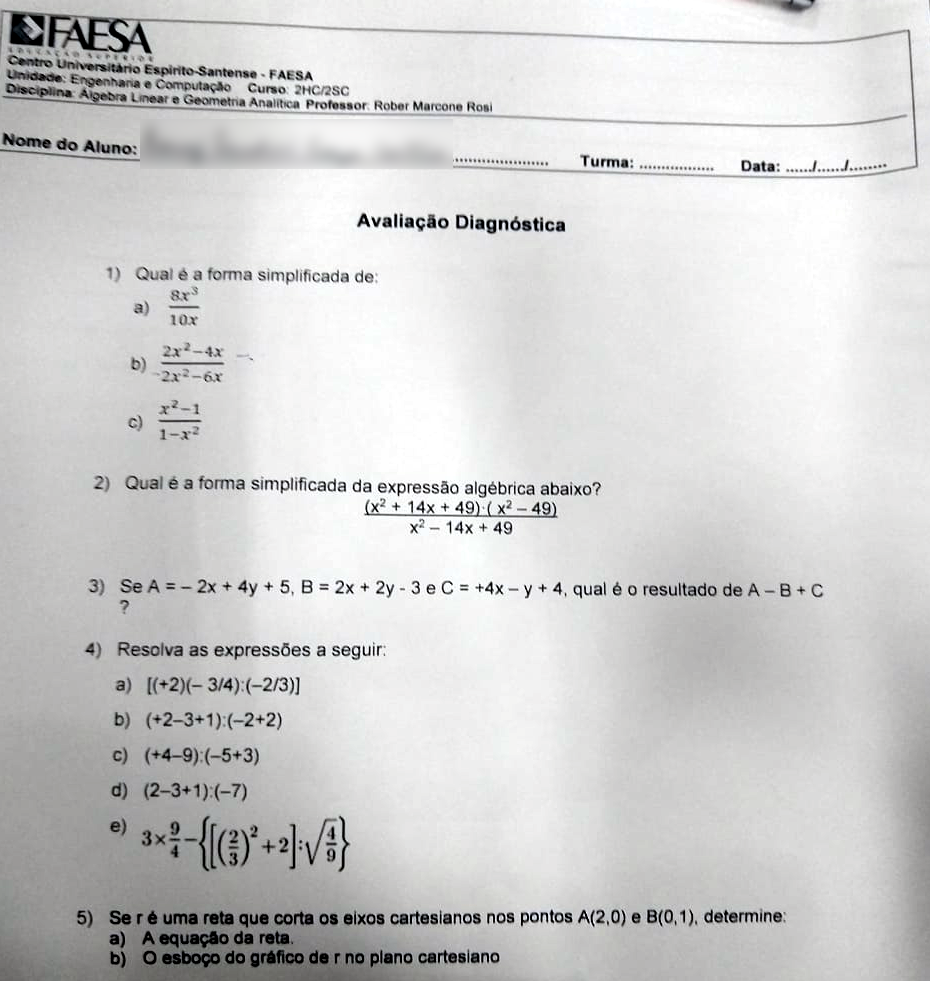
\includegraphics[scale=0.3]{imagens/diag_algebra.png}
    %
    %\footnotesize{Fonte:}
  \end{center}
\end{figure}


%%%%%%%%%%%%%%%%%%%%%%%%%%%%%%%%%%%%%%%%%%%%%%%%%%%%%%%%%%%%%%%%%%%%%%%%%%%%%%%%%
%%%%%%%%%%%%%%%%%%%%%%%%%%%%%%%%%%%%%%%%%%%%%%%%%%%%%%%%%%%%%%%%%%%%%%%%%%%%%%%%%
%%%%%%%%%%%%%%%%%%%%%%%%%%%%%%%%%%%%%%%%%%%%%%%%%%%%%%%%%%%%%%%%%%%%%%%%%%%%%%%%%
\section{Correção}
\label{correcao}

\paragraph{1) Qual a forma simplificada das expressões abaixo?}

\begin{equation}
  \begin{split}
    \frac{8x^3}{10x} &= \frac{8x^{\cancel{3}}}{10\cancel{x}} = \frac{4x^2}{5}
  \end{split}
\end{equation}

\begin{equation}
  \begin{split}
    \frac{2x^2 - 4x}{2x^2 - 6x} &= \frac{2x(x-2)}{2x(x-3)} = \frac{\cancel{2x}(x-2)}{\cancel{2x}(x-3)} = \frac{x-2}{x-3}
  \end{split}
\end{equation}

\begin{equation}
  \begin{split}
    \frac{x^2 - 1}{1- x^2} &= \frac{x^2 - 1^2}{1^2 - x^2} = \frac{(x+1)(x-1)}{(1+x)(1-x)} = \frac{\cancel{(x+1)}(x-1)}{\cancel{(1+x)}(1-x)}\\
                           &= \frac{x-1}{1-x} = \frac{x-1}{-x+1} = \frac{x-1}{-1(x-1)} = \frac{\cancel{x-1}}{-1\cancel{(x-1)}}\\
                           &= \frac{1}{-1} = -1
  \end{split}
\end{equation}

\paragraph{2) Qual a forma simplificada da expressão algébrica abaixo?}

\begin{equation}
  \begin{split}
    \frac{(x^2 + 14x + 49)(x^2 - 49)}{x^2 - 14x + 49} &= \frac{(x^2 + 14x + 49)(x^2 - 7^2)}{x^2 - 14x + 49}
    = \frac{(x^2 + 14x + 49)(x + 7)(x-7)}{x^2 - 14x + 49}\\
    &= \frac{(x+7)^2(x + 7)(x-7)}{x^2 - 14x + 49} = \frac{(x+7)^2(x + 7)(x-7)}{(x-7)^2}\\
    &= \frac{(x+7)^2(x + 7)\cancel{(x-7)}}{(x-7)^{\cancel{2}}} = \frac{(x+7)^3}{x-7}
  \end{split}
\end{equation}

\paragraph{3) Qual o resultado de $A - B + C$?}

\begin{equation}
  \begin{split}
    \begin{cases}
      A = & -2x + 4y + 5\\
      B = & 2x + 2y - 3\\
      C = & 4x - y + 4\\
    \end{cases}&\\
    \therefore A-B+C &= -2x + 4y + 5 - (2x + 2y - 3) + 4x - y + 4\\
    &= -2x + 4y + 5 -2x -2y +3  + 4x - y + 4\\
    &= -4x + 4x +4y - 3y + 12\\
    &= y + 12
  \end{split}
\end{equation}

\paragraph{4) Resolva as expressões a seguir:}

\begin{equation}
  \begin{split}
    [(+2)(-3/4):(-2/3)] &= \frac{2 \cdot \frac{-3}{4}}{\frac{-2}{3}} = \frac{\frac{-6}{4}}{\frac{-2}{3}} = \frac{-6}{4} \cdot \frac{3}{-2}
    = \frac{-18}{-8} = \frac{9}{4} = 2.25
  \end{split}
\end{equation}

\begin{equation}
  \begin{split}
    (+2-3+1):(-2+2) &= \frac{2-3+1}{-2+2} = \frac{0}{0} = \text{indeterminado}
  \end{split}
\end{equation}

\begin{equation}
  \begin{split}
    (+4-9):(-5+3) &= \frac{4-9}{-5+3} = \frac{-5}{-2} = 2.5
  \end{split}
\end{equation}

\begin{equation}
  \begin{split}
    (2-3+1):(-7) = \frac{2-3+1}{-7} = \frac{0}{-7} = 0
  \end{split}
\end{equation}

\begin{equation}
  \begin{split}
    3 \times \frac{9}{4} - \left\{ \left[ \left(\frac{2}{3}\right)^2 + 2 \right]:\sqrt{\frac{4}{9}} \right\} &=
    \frac{27}{4} - \left\{ \frac{\left[ \frac{4}{9} + 2 \right]}{\sqrt{\frac{4}{9}}} \right\} = \frac{27}{4}-\left\{\frac{\frac{4 + 18}{9}}{\frac{2}{3}} \right\} = \frac{27}{4} - \left\{ \frac{22}{9} \cdot \frac{3}{2} \right\}\\
    &= \frac{27}{4} - \frac{66}{18}  = \frac{9 \cdot 27 - 2 \cdot 66}{36} = \frac{243-132}{36}\\
    &= \frac{111}{36} = \frac{37}{12} \approx 3.08
  \end{split}
\end{equation}

\paragraph{5) Se $r$ é uma reta que corta os eixos cartesianos nos pontos $A=(2,0)$ e $B=(0,1)$,
determine:}\ \\
a) a equação da reta;\\
b) o esboço do gráfico de $r$ no plano cartesiano.

\begin{equation}
  \begin{split}
    \text{Slope}\ m &= \frac{\Delta y}{\Delta x} = \frac{1-0}{0-2} = \frac{1}{-2} = -0.5\\
    \text{Intercepto-y} &= 1\text{, uma vez que: } B=(0,1) \implies \text{intercepto-y = 1}\\
    \therefore r &= f(x) = -0.5x + 1
  \end{split}
\end{equation}

\begin{figure}[H]
  \begin{center}
    \caption{Gráfico de $r = f(x) = -0.5x + 1$}
    \label{fig:reta-r}
    %\fbox{\includegraphics[scale=1]{imagens/}}
    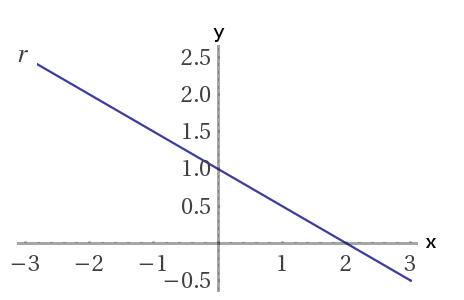
\includegraphics[scale=0.5]{imagens/reta_r.png}
    %
    %\footnotesize{Fonte:}
  \end{center}
\end{figure}


%%%%%%%%%%%%%%%%%%%%%%%%%%%%%%%%%%%%%%%%%%%%%%%%%%%%%%%%%%%%%%%%%%%%%%%%%%%%%%%%%
%%%%%%%%%%%%%%%%%%%%%%%%%%%%%%%%%%%%%%%%%%%%%%%%%%%%%%%%%%%%%%%%%%%%%%%%%%%%%%%%%
%\subsection{}
%\label{}


%%%%%%%%%%%%%%%%%%%%%%%%%%%%%%%%%%%%%%%%%%%%%%%%%%%%%%%%%%%%%%%%%%%%%%%%%%%%%%%%%
%\subsubsection{}
%\label{}




%%%%%%%%%%%%%%%%%%%%%%%%%%%%%%%%%%%%%%%%%%%%%%%%%%%%%%%%%%%%%%%%%%%%%%%%%%%%%%%%%
%%%%%%%%%%%%%%%%%%%%%%%%%%%%%%%%%%%%%%%%%%%%%%%%%%%%%%%%%%%%%%%%%%%%%%%%%%%%%%%%%
%%%%%%%%%%%%%%%%%%%%%%%%%%%%%%%%%%%%%%%%%%%%%%%%%%%%%%%%%%%%%%%%%%%%%%%%%%%%%%%%%
%%%%%%%%%%%%%%%%%%%%%%%%%%%%%%%%%%%%%%%%%%%%%%%%%%%%%%%%%%%%%%%%%%%%%%%%%%%%%%%%%
%%%%%%%%%%%%%%%%%%%%%%%%%%%%%% TERMINA O DOCUMENTO %%%%%%%%%%%%%%%%%%%%%%%%%%%%%%
%%%%%%%%%%%%%%%%%%%%%%%%%%%%%%%%%%%%%%%%%%%%%%%%%%%%%%%%%%%%%%%%%%%%%%%%%%%%%%%%%
%%%%%%%%%%%%%%%%%%%%%%%%%%%%%%%%%%%%%%%%%%%%%%%%%%%%%%%%%%%%%%%%%%%%%%%%%%%%%%%%%
%%%%%%%%%%%%%%%%%%%%%%%%%%%%%%%%%%%%%%%%%%%%%%%%%%%%%%%%%%%%%%%%%%%%%%%%%%%%%%%%%
%%%%%%%%%%%%%%%%%%%%%%%%%%%%%%%%%%%%%%%%%%%%%%%%%%%%%%%%%%%%%%%%%%%%%%%%%%%%%%%%%
\end{document}









